\documentclass{standalone}

\usepackage{tikz} % Allows creation of tikz pictures
\usetikzlibrary{arrows,shapes,snakes}

\begin{document}
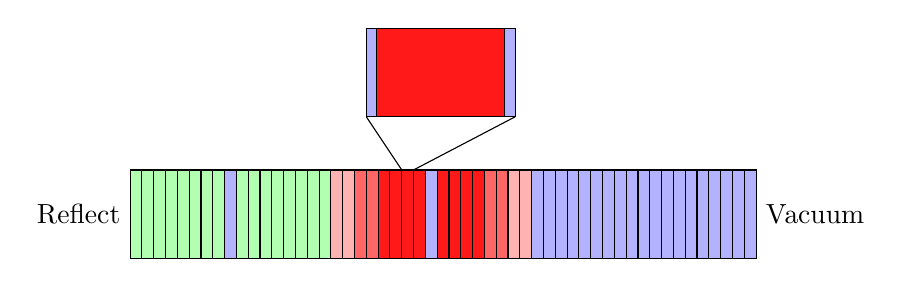
\begin{tikzpicture}[scale=1.5, every node/.style={scale=1}]
    \foreach \x in {0,.1,...,1.7}
    \filldraw[xshift=\x cm,fill=green!30!white,draw=black] (0,0) 
    rectangle (0.1,.75);
    \foreach \x in {1.7,1.8,...,3.4}
    \filldraw[xshift=\x cm,fill=red!30!white,draw=black] (0,0) 
    rectangle (0.1,.75);
    \foreach \x in {1.9,2.0,...,3.2}
    \filldraw[xshift=\x cm,fill=red!60!white,draw=black] (0,0) 
    rectangle (0.1,.75);
    \foreach \x in {2.1,2.2,...,2.9}
    \filldraw[xshift=\x cm,fill=red!90!white,draw=black] (0,0) 
    rectangle (0.1,.75);
    \foreach \x in {3.4,3.5,...,5.3}
    \filldraw[xshift=\x cm,fill=blue!30!white,draw=black] (0,0) 
    rectangle (0.1,.75);
    \foreach \x in {0.8,2.5}
    \filldraw[xshift=\x cm,fill=blue!30!white,draw=black] (0,0) 
    rectangle (0.1,.75);
    \draw (5.3,.375) node[right] {Vacuum};
    \draw (0,.375) node[left] {Reflect};
    % Make zoom
    \draw (2,1.2) -- (2.3,0.75) (2.4,0.75) -- (3.26,1.2);
    \filldraw[xshift=2 cm, yshift=1.2cm,fill=blue!30!white,draw=black] (0,0) 
    rectangle (.09,.75);
    \filldraw[xshift=2.09 cm,yshift=1.2cm, fill=red!90!white,draw=black] (0,0) 
    rectangle (1.17,.75);
    \filldraw[xshift=3.17 cm,yshift=1.2cm, fill=blue!30!white,draw=black] (0,0) 
    rectangle (.09,.75);
\end{tikzpicture}
\end{document}